\documentclass[12pt,a4paper]{report}
\usepackage{dissertation}
\makeglossaries
\makeindex

%\logo{EAAD}{Escola de Arquitetura, Arte e Design}{}
%\logoB{EAAD}{Escola de Arquitetura, Arte e Design}{}

%\logo{EC}{Escola de Ciências}{}
%\logoB{EC}{Escola de Ciências}{}

%\logo{ED}{Escola de Direito}{}
%\logoB{ED}{Escola de Direito}{}

\logo{EE}{Escola de Engenharia}{}
\logoB{EE}{Escola de Engenharia}{}

%\logo{EEG}{Escola de Economia e Gestão}{}
%\logoB{EEG}{SEscola de Economia e Gestão}{}

%\logo{ELACH}{Escola de Letras, Artes e Ciências Humanas}{}
%\logoB{ELACH}{Escola de Letras, Artes e Ciências Humanas}{}

%\logo{EM}{Escola de Medicina}{}
%\logoB{EM}{Escola de Medicina}{}

%\logo{EP}{Escola de Psicologia}{}
%\logoB{EP}{Escola de Psicologia}{}

%\logo{ESE}{Escola Superior de Enfermagem}{}
%\logoB{ESE}{Escola Superior de Enfermagem}{}

%\logo{I3Bs}{Instituto de Investigação em Biomateriais,}{Biodegradáveis e Biomiméticos}
%\logoB{I3Bs}{Instituto de Investigação em Biomateriais,}{Biodegradáveis e Biomiméticos}

%\logo{ICS}{Instituto de Ciências Sociais}{}
%\logoB{ICS}{Instituto de Ciências Sociais}{}

%\logo{IE}{Instituto de Educação}{}
%\logoB{IE}{Instituto de Educação}{}

\author{Nome completo do autor}

\titleA{Título Título Título Título Título Título}
\titleB{Título Título Título Título Título}
\titleC{Título Título Título Título}

\masters{Mestrado em Engenharia Informática}
%\area{Área de especialização}
\supervisor{Nome do Orientador}
\cosupervisor{Nome do Coorientador}

\begin{document}
\setlength{\parindent}{0em}

%-- Covers
\begin{titlepage}
\color{PANTONECoolGray7C}
\thelogo
\leading{20.4pt}
{\Large
\theauthor
\\
%
\\
\textbf{\thetitleA}
\\
\textbf{\thetitleB}
\\
\textbf{\thetitleC}
}

\vspace*{\fill}
{\footnotesize \myear}
\end{titlepage}

\null
\thispagestyle{empty}
\pagecolor{PANTONECoolGray7C}
\afterpage{\nopagecolor}
\newpage

\begin{titlepage}
\color{PANTONECoolGray7C}
\thelogoB
\leading{20.4pt}
{\Large
\theauthor
\\
%
\\
\textbf{\thetitleA}
\\
\textbf{\thetitleB}
\\
\textbf{\thetitleC}
}

\vspace{55.2mm}
\leading{16.8pt}
{\large
Dissertação de Mestrado
\\
\themasters
\\
\thearea
Trabalho efetuado sob a orientação de
\\
\textbf{\thesupervisor}
\\
\thecosupervisor}

\vspace*{\fill}
{\footnotesize \myear}
\end{titlepage}

%-- Document setup
\newgeometry{right=25mm, left=25mm, top=25mm, bottom=25mm}
\pagenumbering{roman}

\setlength{\parskip}{0pt}
\setlength{\parindent}{1.5em}

%-- Preamble
\chapter*{Direitos de Autor e Condições de Utilização do Trabalho por Terceiros}
\setlength{\parskip}{1em}
\noindent
Este é um trabalho académico que pode ser utilizado por terceiros desde que respeitadas as regras e boas práticas internacionalmente aceites, no que concerne aos direitos de autor e direitos conexos.

\noindent
Assim, o presente trabalho pode ser utilizado nos termos previstos na licença abaixo indicada.

\noindent
Caso o utilizador necessite de permissão para poder fazer um uso do trabalho em condições não previstas no licenciamento indicado, deverá contactar o autor, através do RepositóriUM da Universidade do Minho.

\section*{Licença concedida aos utilizadores deste trabalho:}

\textit{[Caso o autor pretenda usar uma das licenças Creative Commons, deve escolher e deixar apenas um dos seguintes ícones e respetivo lettering e URL, eliminando o texto em itálico que se lhe segue. Contudo, é possível optar por outro tipo de licença, devendo, nesse caso, ser incluída a informação necessária adaptando devidamente esta minuta]}

\noindent
\includegraphics[]{images/CCBY.png}
\\
\textbf{CC BY}
\\
\url{https://creativecommons.org/licenses/by/4.0/}
\textit{[Esta licença permite que outros distribuam, remixem, adaptem e criem a partir do seu trabalho, mesmo para fins comerciais, desde que lhe atribuam o devido crédito pela criação original. É a licença mais flexível de todas as licenças disponíveis. É recomendada para maximizar a disseminação e uso dos materiais licenciados.]}

%--

\noindent
\includegraphics[]{images/CCBYSA.png}
\\
\textbf{CC BY-SA}
\\
\url{https://creativecommons.org/licenses/by-sa/4.0/}
\textit{[Esta licença permite que outros remisturem, adaptem e criem a partir do seu trabalho, mesmo para fins comerciais, desde que lhe atribuam o devido crédito e que licenciem as novas criações ao abrigo de termos idênticos. Esta licença costuma ser comparada com as licenças de software livre e de código aberto «copyleft». Todos os trabalhos novos baseados no seu terão a mesma licença, portanto quaisquer trabalhos derivados também permitirão o uso comercial. Esta é a licença usada pela Wikipédia e é recomendada para materiais que seriam beneficiados com a incorporação de conteúdos da Wikipédia e de outros projetos com licenciamento semelhante.]}

%--

\noindent
\includegraphics[]{images/CCBYND.png}
\\
\textbf{CC BY-ND}
\\
\url{https://creativecommons.org/licenses/by-nd/4.0/}
\textit{[Esta licença permite que outras pessoas usem o seu trabalho para qualquer fim, incluindo para fins comerciais. Contudo, o trabalho, na forma adaptada, não poderá ser partilhado com outras pessoas e têm que lhe ser atribuídos os devidos créditos.]}

%--

\noindent
\includegraphics[]{images/CCBYNC.png}
\\
\textbf{CC BY-NC}
\\
\url{https://creativecommons.org/licenses/by-nc/4.0/}
\textit{[Esta licença permite que outros remisturem, adaptem e criem a partir do seu trabalho para fins não comerciais, e embora os novos trabalhos tenham de lhe atribuir o devido crédito e não possam ser usados para fins comerciais, eles não têm de licenciar esses trabalhos derivados ao abrigo dos mesmos termos.]}

%--

\noindent
\includegraphics[]{images/CCBYNCSA.png}
\\
\textbf{CC BY-NC-SA}
\\
\url{https://creativecommons.org/licenses/by-nc-sa/4.0/}
\textit{[Esta licença permite que outros remisturem, adaptem e criem a partir do seu trabalho para fins não comerciais, desde que lhe atribuam a si o devido crédito e que licenciem as novas criações ao abrigo de termos idênticos.]}

%--

\noindent
\includegraphics[]{images/CCBYNCND.png}
\\
\textbf{CC BY-NC-ND}
\\
\url{https://creativecommons.org/licenses/by-nc-nd/4.0/}
\textit{[Esta é a mais restritiva das nossas seis licenças principais, só permitindo que outros façam download dos seus trabalhos e os compartilhem desde que lhe sejam atribuídos a si os devidos créditos, mas sem que possam alterá- los de nenhuma forma ou utilizá-los para fins comerciais.]}

\setlength{\parskip}{0em}
\chapter*{Agradecimentos}
\setlength{\parskip}{1em}

A consolidação do atual trabalho servirá, expectavelmente, como um marco da fase de estudo que, mais ou menos duradoura, a todos marca.

Alcançar este ponto é prova não apenas do meu esforço, mas de todos os que sempre me apoiaram, em especial os meus pais. A educação e formação que me incutiram e os ideais que me constituem são, por base, fruto da sua dedicação e carinho. 

Também a boa disposição e companheirismo inabaláveis da minha irmã não poderiam ser ignorados.

De igual forma agradeço à minha avô, que forneceu os momentos mais ternos da minha infância e juventude, e que sempre teve confiança nas minhas capacidades. 

Agradeço, aos professores e escolas que me formaram durante o caminho e serviram como alicerces da minha aprendizagem. Ao meu orientador, prof. José João por ter sido um guia paciente e elucidador durante este ano de trabalho, pelas inúmeras ideias que sugeriu e tornaram este um trabalho mais interessante, pelas palavras de experiência e as oportunidades que forneceu.

Aos meus amigos que me acompanharam durante este percurso, que forneceram momentos insubstituíveis e laços preciosos, uma saudação calorosa.

A todos os que direta ou indiretamente me marcaram, obrigado!

\setlength{\parskip}{0em}
\chapter*{Declaração de Integridade}
\setlength{\parskip}{1em}
\noindent
Declaro ter atuado com integridade na elaboração do presente trabalho académico e confirmo que não recorri à prática de plágio nem a qualquer forma de utilização indevida ou falsificação de informações ou resultados em nenhuma das etapas conducente à sua elaboração.

\noindent
Mais declaro que conheço e que respeitei o Código de Conduta Ética da Universidade do Minho.


\phantom{space for signature}

\noindent
Universidade do Minho, Braga, \myear

\vspace{25mm}
\noindent\theauthor
\setlength{\parskip}{0em}
\chapter*{Resumo}

\newacronym{ocr}{OCR}{reconhecimento óptico de caracteres}
\newacronym{gui}{GUI}{graphic user interface}

A digitalização de documentos permitiu uma nova forma de salvaguardar informação para a posteridade, evitando a sua perda pelo deterioramento físico destes. De forma a posteriormente transcrever estes documentos, permitindo uma consulta, processamento e manipulação mais simples, o uso de software de \acrshort{ocr} é essencial. Esta tecnologia é, no entanto, dependente em diferentes níveis das características do seu alvo, nomeadamente: qualidade da imagem, complexidade da estrutura do documento, linguagem do texto. 

Documentos mais antigos, em especial jornais por apresentarem estruturas mais complexas, apresentam por este motivo resultados que diferem bastante do seu conteúdo original; tanto a nível do texto reconhecido, como da sua organização para os diferentes outputs disponíveis (ex.: txt simples). A tarefa de extrair informação destes documentos, como por exemplo o isolamento e extração de artigos, torna-se assim complexa e propensa a erros. 

Este trabalho propõe então a criação de uma ferramenta ou um conjunto de ferramentas que permitam auxiliar o processo de extração de conteúdo de documentos, primeiramente mas não exclusivamente, mais antigos e estruturados, com especial foco em jornais. A solução do projeto pretende então ser capaz de detetar e lidar com os diferentes pontos de risco nestes documentos: qualidade da imagem, erros nos resultados de \acrshort{ocr}, segmentação e organização do documento, criação do output organizado. 

Diferentes alternativas para \acrshort{ocr} assim como métodos de tratamento destes problemas serão estudados, comparados, e implementados, de forma a encontrar a melhor solução para a resolução deste problema. O produto final implementado será composto por 3 componentes principais: um Toolkit com ênfase na manipulação de resultados OCR, mas também de tratamento de imagem; uma aplicação do Toolkit na forma de pipeline de OCR, que também explora ferramentas externas; um Editor de resultados OCR, também aplicação do Toolkit, que facilite a manipulação destes devido ao seu aspeto visual, e o teste das outras componentes. 

Na base desta solução, tem o módulo OCR Tree que procura servir como representação universal dos resultados de OCR


\paragraph{Palavras-chave} OCR, Digitalização, Documentos estruturados, Documentos antigos, Segmentação de documentos, Tratamento de imagem, Modernização de texto

\cleardoublepage

\chapter*{Abstract}

The digitization of documents has opened a new way of preserving information for posterity, avoiding its loss through their physical decay. To allow the transcription of these documents, enabling an easier search, indexation and manipulation of them, the use of \acrshort{ocr} software is essential. This technology is, however, dependent in many ways of the characteristics of its target, namely: the quality of the image, the complexity of the document's structure, the text's language. 

Older documents, especially newspapers for having complex structures, result in poor transcriptions that differ from their original content, both in the recognized text, and in the organization of the available final outputs (ex.: simple txt).
Extracting information from these documents, for example, the isolation and extraction of articles, becomes thus a complex and error prone task. 

Therefore, this work aims to create a tool, or a toolkit, that can assist in the process of content extraction from documents, primarily though not exclusively, that are older and structured, specializing in newspapers. The proposed pipeline should then be able to detect and fix potential problems in these documents: image quality, \acrshort{ocr} results errors, segmentation and document organization, restructured output generation.

Different \acrshort{ocr} alternatives, as well as different methods of dealing with these problems, will be studied, compared, and implemented, to find the best solution for the task at hand. The final product will be composed of 3 main components: a Toolkit with emphasis on the manipulation of OCR results, but also image processing; an application of said Toolkit in the shape of an OCR pipeline, which will also explore other external tools; an OCR results Editor, also an application of the Toolkit, which eases the manipulation of these thanks to its visual approach, as well as the testing of the other components.

The basis of this solution is the OCR Tree module, which aims to serve as an universal representation of OCR results.


\paragraph{Keywords} OCR, Digitalization, Structured documents, Old documents, Document segmentation, Image treatment, Text modernization

\cleardoublepage


\phantomsection
\tableofcontents

\cleardoublepage
\listoffigures

% List of tables
\listoftables
\clearpage

% Acronyms
\printglossary[type=\acronymtype,nonumberlist, title={Acrónimos}]

% Glossary
\printglossary[title={Glossário}, nonumberlist]

\cleardoublepage
\pagenumbering{arabic}

%-- Dissertation 
\part{Material Introdutório}

\chapter{Introdução}
\label{cap_introducao}

Neste capítulo, será realizada uma introdução ao problema que o projeto tenciona abordar, composta por uma contextualização do seu estado atual e os desafios que sobre este são impostos. Além disso, os objetivos do trabalho serão listados e será descrita a estrutura do documento.

%Contexto, motivação, principais objetivos.
\section{Enquadramento e motivação}


A digitalização tem um papel fundamental na conservação, disponibilização e proliferação de documentos físicos, não só contemporâneos, mas também de eras anteriores à revolução da informação. Esta tecnologia, acoplada a ferramentas de \acrshort{ocr}, veio trazer uma facilidade de navegação, consulta e manipulação destes documentos que anteriormente não era possível.

A eficácia de \acrshort{ocr} é no entanto dependente de vários fatores nas imagens ou ficheiros alvo: a qualidade das imagens, como a resolução, estado do documento, coloração, qualidade/tipo de escrita; a estrutura dos documentos - quanto mais complexo, mais difícil é obter a informação de forma automática mantendo 
 a congruência original -; linguagem do texto, sendo que por vezes diferentes tecnologias, como por exemplo \textbf{Tesseract}, procuram verificar a sua confiança na deteção com o vocabulário conhecido, o qual pode não coincidir com a época de produção do documento; entre outras. 

Estas dependências são especialmente notórias quando se envolvem documentos mais antigos, os quais podem, além de apresentar envelhecimento causado pelo tempo e danos pelas condições de armazenamento, devido às limitações tecnológicas assim como por vezes à falta de convenções de formatação dos documentos, não dispor de uma consistência no formato e texto (estrutura, alinhamento, dimensões dos caracteres, fonte de texto consistente, etc.) usual nos documentos atuais. Estes fatores resultam então num reconhecimento de texto não tão satisfatórios. 

Estes documentos antigos são mais comummente, mas não exclusivamente, reconhecidos como anteriores à era digital, sendo que o foco de trabalho será maioritariamente dirigido a documentos desta época, como jornais, revistas e outros, do século passado ou anteriores. 
Em especial documentos com estruturas complexas, como é o caso de jornais, onde é possível a segmentação em diferentes partes com conteúdo e propósito distinto e, ao mesmo tempo, uma ordem de leitura complexa i.e., não segue apenas regras simples de posição do conteúdo (texto da esquerda antes do texto da direita e cima antes de baixo), exigindo também noção das características e relação do conteúdo. 

Mesmo para ficheiros do tipo \textbf{hOCR} ou \textbf{PDF}, que já passaram por um processo de reconhecimento de texto, a complexidade da estrutura dos documentos originais ou problemas nos elementos que contém o texto (como por exemplo elementos sobrepostos ou que se intersetam) dificultam a extração e interpretação do seu conteúdo, podendo ser facilmente perdida a lógica original.

Por estas razões, seria útil uma ferramenta que permita uma deteção e tratamento destes documentos de forma automática e de uso simples, permitindo um certo nível de configuração para adaptação entre tipos de documentos com características bem definidas e distintas. 

O presente documento pretende então servir como um estudo dos desafios apresentados por estes tipos de documentos perante \acrshort{ocr}, assim como a procura de soluções para a melhoria dos resultados na deteção  e extração de texto e assim criar uma ferramenta que torne o processo de extração de informação destes tipos de documentos mais simples e fiável. 

Como trabalho complementar, é proposta a implementação de um método de modernização do conteúdo extraído, envolvendo a criação de uma ferramenta capaz de criar dicionários entre diferentes iterações de uma mesma linguagem. 

\section{Objetivos}
\label{section_objetivos}

O principal objetivo deste trabalho é a realização de um estudo sobre os problemas apresentados à extração de conteúdo de documentos de estrutura complexa - mantendo 
a sua lógica original -, assim como a implementação de uma solução para resolver ou mitigar estes desafios, aumentando a confiança na informação extraída. 
Em termos dos casos alvo do trabalho, será prioridade o estudo de jornais com texto máquina. Tal deve-se ao facto de jornais serem um particular tipo de documento que apresenta mais dificuldades e se encontra em maior procura de soluções e, texto máquina por ser mais comum para este tipo de documento. Esta segunda restrição é menos relevante pois não é uma dificuldade do trabalho e pode ser resolvida perante a escolha da tecnologia de reconhecimento utilizada.

Especificando, os objetivos do trabalho são:
\begin{itemize}
    \item Estudar os diferentes softwares de \acrshort{ocr} disponíveis e as diferenças entre estes.
    \item Estudar as dificuldades que documentos podem apresentar no processo de reconhecimento de texto.
    \item Estudar o trabalho desenvolvido sobre a área de tratamento de imagem, identificação de tipo de documento, segmentação de documentos, algoritmos de cálculo da ordem de leitura, melhoria de resultados de \acrshort{ocr} e métricas de validação de resultado \acrshort{ocr}.
    \item Estudar trabalhos com âmbito similar ou relacionado ao presente.
    \item Implementação de um conjunto de ferramentas dirigidas à solução dos problemas propostos.
    \item Implementação de uma ferramenta em formato \acrshort{gui} e comando de consola que aplique uma pipeline cujo input seria um ficheiro - imagem, pdf, hOCR -, identifique e trate de problemas deste se necessário para melhorar os resultados de \acrshort{ocr} e, por fim, devolva um output que mantenha a lógica e conteúdo do documento original.
    \item Secundário : ferramenta para criação de dicionário de diferentes versões de uma linguagem para: modernização de texto; léxico de motor \acrshort{ocr}. Ferramenta tem como input duas versões de um documento na mesma linguagem mas iterações diferentes e dá como output um dicionário entre as versões.
    \begin{itemize}
        \item Estudo sobre criação de léxicos e alinhamento de documentos.
    \end{itemize}
\end{itemize}



\section{Estrutura da dissertação}

Esta dissertação segue a seguinte estrutura:

\begin{itemize}
    \item Capítulo \ref{cap_introducao}: Breve contextualização sobre o tema proposto, as dificuldades impostas por documentos estruturados e com digitalizações ou condições físicas degradadas, nos resultados \acrshort{ocr}, e a utilidade de uma ferramenta para o tratamento destas. Além disso foram listados os objetivos do trabalho.

    \item Capítulo \ref{cap_estado_arte}: Estudo sobre o estado da arte nos tópicos relacionados ao tema da dissertação, as suas dificuldades e soluções destas; estudo de trabalho anteriormente realizado com âmbito similar ao atual ou técnicas relevantes para a construção da solução do problema.

    \item Capítulo \ref{cap_problema}: Listagem dos diferentes problemas que a solução irá abranger e os desafios que estes apresentam. Apresentação do desenho da solução.

    \item Capítulo \ref{cap_contribuicao}: Descrição da solução e ferramentas implementadas.

    \item Capítulo \ref{cap_aplicacoes}: Apresentação e estudo dos resultados do trabalho realizado.

    \item Capítulo \ref{cap_conclusao}: Reflexão sobre o trabalho realizado, os resultados e a experiência obtida, assim como uma breve exploração de caminhos para trabalho futuro do projeto. 

    \item Capítulo \ref{cap_planeamento}: No último capítulo é explicado o plano de desenvolvimento da dissertação.
\end{itemize}

\chapter{Estado da arte}

Estado da arte revisto; trabalho relacionado.

\section{Citações}
Exemplo de uma citação: \cite{GRM97}, cf. esta entrada em \texttt{dissertation.bib}.
Outra forma de citar \citep{KeR88}.

\section{Expressões matemáticas}
A equivalência massa-energia é descrita pela famosa equação
\begin{equation}
E=mc^2
\end{equation}
descoberta em 1905 por Albert Einstein.
Em unidades naturais ($c = 1$), a fórmula expressa a identidade
\[
E=m
\]

\section{Notas de rodapé}
Este é um exemplo de uma nota de rodapé\footnote{The quick brown fox jumps over the lazy dog.}.

\section{Acrónimos e Glossário}
\newacronym{gcd}{MDC}{
Máximo Divisor Comum}
\newacronym{lcm}{MMC}{Mínimo múltiplo comum}
\newglossaryentry{maths}
{
    name=matemática,
    description={Matemática é o que os matemáticos fazem}
}
\newglossaryentry{latex}
{
    name=latex,
    description={É uma linguagem especialmente adequada para
documentos científicos}
}
\newglossaryentry{formula}
{
    name=fórmula,
    description={Expressão matemática}
}

Dado um conjunto de números, existem métodos elementares para calcular
seu \acrlong{gcd}, que é abreviado como \acrshort{gcd}. Este processo
é semelhante ao usado para o \acrfull{lcm}.

O \Gls{latex} é especialmente adequado
para documentos que incluam \gls{maths}. \Glspl{formula} são corretamente e facilmente renderizados a partir do momento que nos habituamos aos comandos.

\section{Índice}

Neste exemplo, várias palavras-chave\index{palavras-chave} importantes serão usadas pelo que merecem aparecer no Índice\index{Índice}.

Os termos no índice também podem ser aninhados \index{Índice!aninhados}.

Cf. o ficheiro \texttt{dissertation.bib} para ver algumas definições como \uminho{UMinho}.

\chapter{O problema e os seus desafios}
\label{cap_problema}


Neste capítulo, é feita uma síntese dos desafios do problema e uma discussão sobre a solução desenhada até ao momento para concretizar os objetivos definidos.

\section{Desafios}

No capítulo \ref{cap_estado_arte}, realizou-se um estudo abrangente sobre o estado da arte no que toca a projetos que utilizem \acrshort{ocr} e trabalhos relacionados com os objetivos listados para este projeto (\ref{section_objetivos}).  Através deste estudo, foi possível extrair um leque de problemas detetados na utilização de reconhecimento de texto em documentos, de forma generalizada ou para tipos específicos como é o caso deste trabalho. Em suma, os principais desafios são:
\begin{itemize}
    \item \textbf{Problemas de imagem} : tanto na imagem de input, como no documento original. Ex.: ruído, baixa resolução, má iluminação.
    \item \textbf{Problemas de reconhecimento} : estes são muitas vezes derivados do conjunto anterior, mas outras questões como léxico no documento desconhecido pelo motor OCR ou estruturas complexas podem provocar erros no reconhecimento.
    \item \textbf{Problemas nos resultados} : consideremos estes os problemas sobre as entidades reconhecidas pelo software, tanto o texto que em muitos casos apresenta erros como os próprios contentores em que estes são incluídos.
    \item \textbf{Problemas na extração de conteúdo} : no processo de criação de output, por vezes questões como a ordem de leitura dos blocos identificados, ou reposição de elementos não texto têm de ser abordados.
    \item \textbf{Validação da implementação} : de forma a verificar a eficácia da solução criada, geralmente datasets de teste e casos de estudo relevantes têm de ser criados.
\end{itemize}


\section{Plano da Solução}
\begin{wrapfigure}{r}{0.3\textwidth}
    \includegraphics[width=0.25\textwidth]{images//diagramas/pipeline_geral.png}
    \caption{Pipeline da solução}
    \label{fig:pipeline_geral}
\end{wrapfigure}
Durante o estudo do estado da arte, tornou-se evidente que a maioria dos trabalhos com vista em extrair ou corrigir a extração de documentos utilizando reconhecimento de texto, de forma a manter o conteúdo e lógica original, seguem uma metodologia semelhante: uma primeira fase de pré processamento da imagem de input; possível segmentação da imagem entre texto e não texto; reconhecimento de texto; pós processamento do texto; possível pós processamento para segmentação de conteúdo específico de um tipo de ficheiro, como artigos, ou para reorganização dos resultados (ordem de leitura); criação de output.

Partindo desta base, a figura \ref{fig:pipeline_geral} representa o fluxo da solução planeada atualmente. 

A pipeline começa com a introdução de um input, podendo este ser sujeito de reconhecimento de texto, no caso de ser uma imagem, ou já possuir os resultados de reconhecimento, como hOCR. No caso de uma imagem, antes de ser aplicado o software de OCR, será realizado pré processamento da imagem para aumentar a chance de bons resultados de OCR.

Os resultados de OCR são então convertidos para uma estrutura de dados genérica, de modo a englobar os diferentes tipos de resultados possíveis de diferentes tipos de ficheiros ou motores de OCR. Em diante, esta estrutura será usada nos módulos que utilizam os resultados de OCR.

Depois, passa-se por um processo de pós processamento básico dos resultados de OCR. Tal tem o intuito de corrigir erros menos severos no que toca às \textit{bounding boxes} dos resultados e lixo reconhecido pelo motor.

Uma análise dos resultados limpos é então realizada, extraindo informação sobre o texto reconhecido, estimas do possível layout, erros de reconhecimento, etc.. Com os resultados da análise feita, abre-se a possibilidade de realizar um tratamento de imagem diferente dedicado à resolução de problemas detetados, por exemplo: detetado um \acrshort{dpi} de imagem muito baixo, este é um indicador de que a resolução da imagem poderia ser aumentado para melhorar o reconhecimento, procedimento comum no estudo feito.

Utilizando os resultados da análise, são de pois aplicados algoritmos para extração do conteúdo do documento. Aqui o principal objetivo será o cálculo da ordem de leitura e agrupamento dos elementos em conjuntos como artigos.
Além disso, o objetivo secundário envolvente da modernização de texto poderá nesta etapa ser aplicado.

Finalmente, o output final é gerado. Diferentes formas de output serão disponibilizadas dependendo da estrutura pretendida, por exemplo: markdown ou texto simples no caso de apenas se querer os elementos do texto isolado; html para reconstruir a estrutura do documento original. 



\part{\textit{Core} da Dissertação}

\chapter{Contribuição}
\label{cap_contribuicao}

Nesta secção, será relatado o trabalho realizado no intuito da componente prática do projeto e os resultados. 
% Neste caso, relevante à criação de um \textit{toolkit} e ferramentas para a extração do conteúdo de documentos antigos, em particular jornais, com melhores resultados do que os oferecidos pelas ferramentas de \acrshort{ocr} base e, possibilitando a obtenção da lógica e organização original dos mesmos.

\section{Introdução}
% Ao longo do período de inicialização da dissertação: desde a definição dos objetivos do projeto, aprofundamento da temática e estudo do estado da arte; de forma a simultaneamente acostumar com as tecnologias, assim como ganhar um melhor entendimento sobre os algoritmos a implementar e os desafios apresentados, algum trabalho prático já foi realizado. 
% Este envolve principalmente a criação de uma ferramenta para facilitar a visualização dos resultados de reconhecimento, assim como o debugging destes e alguns algoritmos preliminares para manipulação destes resultados de \acrshort{ocr}.

A discussão sobre o trabalho realizado será estruturada em 3 componentes principais.
\begin{itemize}
	\item Ferramentas do \textit{toolkit} desenvolvidas
	\item Pipeline de aplicação do toolkit
% 	\item GUI de aplicação geral do \textit{toolkit}
	\item GUI editor OCR
\end{itemize}

Para cada uma das secções delimitadas, será dada uma explicação do seu propósito e produto sumariado, procedido por uma discussão mais detalhada dos elementos que a constituem.

De forma geral, o código desenvolvido foi maioritariamente escrito em Python, com algumas instâncias de C.

\section{Ferramentas do \textit{toolkit} desenvolvidas}

\subsection{Introdução}

A componente do \textit{toolkit} foi a premissa base do tema da dissertação. Um conjunto de ferramentas focado na melhoria dos resultados obtidos da aplicação de \acrshort{ocr} em documentos antigos, com especial interesse em jornais. 

Estas ferramentas são então pertinentes para os diversos passos do processo convencional de \acrshort{ocr}, i.e. pré-processamento, OCR e pós-processamento; atendendo tanto a processamento de imagem, processamento de resultados de OCR e texto, e validação de resultados.

Além dos métodos principais criados para a resolução de problemas identificados, é importante realçar certos pontos essenciais que serviram como base para o resto do trabalho. Estes são as estruturas de dados utilizadas para o tratamento dos resultados de OCR.

\subsection{Sumário}

\begin{itemize}\setlength\itemsep{-0.3em}
	\item Estruturas de dados \ref{data_structures}
	\begin{itemize}\setlength\itemsep{-0.3em}
		\item OCR Tree \ref{ocr_tree}
		\item Box \ref{box_data_structure}
	\end{itemize}
	\item Métodos \ref{contribution_methods}
	
	\begin{itemize}\setlength\itemsep{-0.3em}
		\item Processamento de resultados OCR \ref{contribution_ocr_posprocessing}
		
		\begin{itemize}\setlength\itemsep{-0.3em}
			\item Conversão de resultados OCR \ref{ocr_results_conversion}
			\item Debugging \ref{contribution_debugging}
			\item Análise de texto \ref{contribution_text_analyses}
			\item Limpeza de OCR Tree \ref{contribution_clean_ocr}
			\item Categorização de Blocos \ref{contribution_categorize_blocks}
			\item Divisão de blocos \ref{contribution_divide_blocks}
			\item Cálculo de ordem de leitura \ref{contribution_reading_order}
			\item Segmentação de resultados \ref{contribution_result_segmentation}
		\end{itemize}
		
		\item Processamento de imagem \ref{contribution_image_processing}
		\begin{itemize}\setlength\itemsep{-0.3em}
			\item Binarização de imagem
			\item Rotação de imagem
			\item Cálculo de sentido de rotação
			\item Segmentação de documento
			\item Identificação de imagens
			\item Identificação de delimitadores
			\item Divisão de colunas 
		\end{itemize}
		
		\item Processamento de texto \ref{contribution_text_processing}
		\begin{itemize}\setlength\itemsep{-0.3em}
			\item Limpeza de hifenização
		\end{itemize}
		
	\end{itemize}
	
	\item Validação de resultados \ref{contribution_results_validation}
	
\end{itemize}


\subsection{Estruturas de dados}
\label{data_structures}


\subsubsection{OCR Tree}
\label{ocr_tree}

Como o produto final do projeto intende aceitar diferentes tipos de resultados OCR, i.e. resultantes de diferentes motores OCR ou de ficheiros como hOCR que já possuem os resultados, existe uma necessidade de converter estes diferentes formatos num único tipo que mantenha a informação base pretendida.

Estruturas de dados standard como \citep{hocr_doc} ou \citep{alto_doc} apresentam um resultado final semelhante e com capacidade base de armazenamento de meta-dados superior porém, sendo baseados em XML, tornam a sua manipulação mais complexa e, em múltiplos casos a informação proporcionada é além do necessário ou gera conclusões erradas quando gerado de output automático (ex.: atribuição de classes caption a blocos que são títulos). Assim sendo, embora tenha sido desenvolvido um conversor de, e para HOCR, para o atual projeto, optou-se pela criação de uma estrutura de dados própria.

Deste modo, tomando como inspiração os atributos dos resultados do Tesseract no modo de dicionário \citep{tesseract_doc}, foi implementada uma estrutura de dados no formato de árvore de dados.

A escolha de uma estrutura de árvore permite a hierarquização de blocos de acordo com o seu nível, quer exista uma divisão de nível à partida, como é o caso do Tesseract que segue: página $\longrightarrow$ bloco $\longrightarrow$ parágrafo $\longrightarrow$ linha $\longrightarrow$ palavra; ou apenas um único nível, semelhante ao Keras-OCR.

Todos os algoritmos desenvolvidos, inclusive os métodos para visualização (métodos de debugging e GUI desenvolvido), assumem e trabalham com os dados de OCR no formato desta estrutura de dados.

As características mais relevantes desta estrutura são:

\begin{itemize}\setlength\itemsep{-0.3em}
	\item \textbf{Level} : Nível/altura do nodo.
	\begin{itemize}\setlength\itemsep{-0.3em}
		\item documento : 0
		\item página 	: 1
		\item bloco		: 2
		\item parágrafo : 3
		\item linha 	: 4
		\item palavra	: 5
	\end{itemize}\setlength\itemsep{-0.3em}
	\item \textbf{(page|block|par|line|word)\_num}: Identificação da ordem (dentro de outras caixas(ex.: linha), se aplicável)
	\item \textbf{text} : Texto do bloco, normalmente apenas preenchido ao nível da palavra
	\item \textbf{conf} : Confiança no texto
	\item \textbf{id}
	\item \textbf{type} : Tipo do bloco, ex.: delimitador, título
	\item \textbf{children}
	\item \textbf{box}: Bounding box do nodo, representado pela estrutura de dados Box, que também possui métodos para transformações e verificações geométricas ou de características.
	\item Características de texto: ex.: texto iniciado (start\_text); texto não terminado (end\_text).
\end{itemize}

%% TODO : Ilustracao de uso de arvore OCR para demonstrar diferentes niveis de um documento

Construtores da classe são capazes de admitir outros atributos não base de modo a expandir a utilidade da estrutura. Construtores disponíveis: iniciação por argumentos, dicionário, ficheiro JSON e ficheiro HOCR.

Da mesma forma, conversores para estes ficheiros compreendidos para iniciação também foram desenvolvidos.

A classe possuí por métodos de transformação e análise sobre a árvore OCR que facilitam a manipulação dos resultados OCR. 

Segue-se uma lista dos métodos mais relevantes disponíveis da classe.

\highlight{id\_boxes}
 
 
\textbf{Descrição:} Adiciona identificador aos blocos.
	
\textbf{Argumentos:}
	\begin{itemize}\setlength\itemsep{-0.3em}
		\item level : lista de níveis onde adicionar identificador
		\item ids (opt): dicionário de ids a utilizar caso não se queira iniciar no 0.
		\item delimiters (opt): flag para identificar delimitadores
		\item area (opt): argumento do tipo Box, que restringe os nodos a identificar a uma dada área
		\item override (opt): flag para reescrever id se já existe.
	\end{itemize}
				
\highlight{calculate\_mean\_height}

\textbf{Descrição:} Calcula a altura média das caixas de um dado nível.
	
\textbf{Argumentos:}
\begin{itemize}\setlength\itemsep{-0.3em}
	\item level : nível a calcular
	\item conf (opt): valor de confiança de texto no caso de apenas serem relevantes caixas com certa confiança (aplicável apenas para nível de texto)
\end{itemize}

	
\highlight{is\_text\_size}

\textbf{Descrição:} Verifica se um nodo se encontra dentro do tamanho de texto.
	
\textbf{Argumentos:}
\begin{itemize}\setlength\itemsep{-0.3em}
	\item text\_size : tamanho de texto a comparar
	\item mean\_height (opt): altura do bloco, caso já tenha sido calculado
	\item range : margem de erro aceitável (relativo)
	\item level : nível das caixas usado caso seja necessário calcular a altura média
	\item conf : confiança do texto a utilizar para calcular a altura média
\end{itemize}

\highlight{is\_empty}

\textbf{Descrição:} Verifica se um nodo é vazio.
	
\textbf{Argumentos:}
\begin{itemize}\setlength\itemsep{-0.3em}
	\item conf : confiança de texto a utilizar para considerar palavras válidas
	\item only\_text : flag que dita se o tipo do bloco influencia o resultado, i.e. blocos de tipo "image" não são vazios
\end{itemize}

	
\highlight{text\_is\_title}

\textbf{Descrição:} Verifica se um nodo é potencial título.
	
\textbf{Algoritmo:} Caixa não é texto vertical e é maior do que o tamanho normal de texto.


\textbf{Argumentos:}
\begin{itemize}\setlength\itemsep{-0.3em}
	\item normal\_text\_size : tamanho de texto considerado como normal
	\item conf : confiança de texto a utilizar para considerar palavras válidas
	\item range : margem de acerto aceitável (relativo)
	\item level : nível usado para calcular o tamanho médio do bloco
\end{itemize}

	
\highlight{is\_delimiter}

\textbf{Descrição:} Verifica se um nodo é potencial delimitador.
	
\textbf{Algoritmo:} Caixa já é do tipo delimitador, ou é vazia e segue a regra:

$ box.width >= box.height*4 || box.height >= box.widht*4 $.


\textbf{Argumentos:}
\begin{itemize}\setlength\itemsep{-0.3em}
	\item conf : confiança de texto a utilizar para considerar palavras válidas
	\item only\_type : flag que dita se usa apenas o tipo do nodo para a verificação
\end{itemize}

	
\highlight{is\_image}

\textbf{Descrição:} Verifica se um nodo é potencial imagem.
	
\textbf{Algoritmo:} Caixa já é do tipo imagem ou, é vazia, não é um delimitador e é 3 vezes mais alta do que o tamanho de texto.


\textbf{Argumentos:}
\begin{itemize}\setlength\itemsep{-0.3em}
	\item conf : confiança de texto a utilizar para considerar palavras válidas
	\item text\_size : tamanho de texto a utilizar para comparação com altura da caixa
	\item only\_type : flag que dita se usa apenas o tipo do nodo para a verificação
\end{itemize}


\highlight{get\_boxes\_in\_area}

\textbf{Descrição:} Obtém todas as caixas numa dada área.


\textbf{Argumentos:}
\begin{itemize}\setlength\itemsep{-0.3em}
	\item area : área de interesse
	\item level : nível dos nodos a ir buscas. Se nível == -1, obtém todos os nodos
	\item conf : confiança de texto a utilizar para considerar nodos válidos
	\item ignore\_type : tipos de nodo a ignorar
\end{itemize}
	
	
\highlight{is\_vertical\_text}

\textbf{Descrição:} Verifica se um nodo é texto vertical.

\textbf{Argumentos:}
\begin{itemize}\setlength\itemsep{-0.3em}
	\item conf : confiança de texto a utilizar para considerar palavras válidas
\end{itemize}
	
\textbf{Algoritmo:}

\begin{algorithm}[H]
	\caption{Verificação de texto vertical}
	\algsetup{linenosize=\tiny}
	\tiny
	\begin{algorithmic}[1]
		\IF{nodo não é vazio}
			\STATE lines
			\IF{len(lines) == 0}
				\RETURN False
			\ENDIF
			\STATE \textit{// Linha única}
			\IF{len(lines) == 1}
				\STATE words
			 \STATE \textit{// Palavra única}
				\IF{len(words) == 1}
					\IF{altura da palavra >= 2 * largura da palavra}
						\RETURN True
					\ENDIF
				\STATE \textit{// Múltiplas palavras} 
				
				\Else
					\STATE \textit{// Verifica se a maioria das palavras coincidem horizontalmente}
					\STATE widest\_word <- calcula palavra mais larga
					\STATE overlapped\_words = 0
					\FOR{word in words}
						\IF{word == widest\_word}
							\STATE continue
						\ENDIF
						\IF{word.box.within\_horizontal\_boxes(widest\_word.box,range=0.1)}
							\STATE overlapped\_words += 1
						\ENDIF
					\ENDFOR
					\IF{overlapped\_words/len(words) >= 0.5}
						\RETURN True
					\ENDIF
					
				\ENDIF
				
			\STATE \textit{// Múltiplas linhas} 
			
			\Else
				\STATE \textit{// Verifica se a maioria das linhas coincidem verticalmente}
				\STATE tallest\_line <- calcula linha mais alta
				\STATE overlapped\_lines = 0
				
				\FOR{line in lines}
					\IF{line == tallest\_line}
						\STATE continue
					\ENDIF
					\IF{line.box.withinvertical\_boxes(tallest\_line.box,range=0.1)}
						\STATE overlapped\_lines += 1
					\ENDIF
				\ENDFOR
				\IF{overlapped\_lines/len(lines) >= 0.5}
					\RETURN True
				\ENDIF
			
			\ENDIF
			
		\ENDIF
		
		\RETURN	False
		
	\end{algorithmic}
\end{algorithm}



\highlight{prune\_children\_area}

\textbf{Descrição:} Atualiza dimensões dos filhos de um nodo para se encaixarem dentro de uma área.


\textbf{Argumentos:}
\begin{itemize}\setlength\itemsep{-0.3em}
	\item area : área de interesse
\end{itemize}


\highlight{boxes\_below}
(método semelhante para as outras direções)

\textbf{Descrição:} Dada uma lista de OCR Tree, devolve aqueles que se encontram por baixo do bloco atual. Os blocos filtrados podem intersetar ou estar dentro do bloco comparado.


\textbf{Argumentos:}
\begin{itemize}\setlength\itemsep{-0.3em}
	\item blocks : lista de blocos a filtrar
\end{itemize}



\highlight{boxes\_directly\_below}
(método semelhante para as outras direções)

\textbf{Descrição:} Dada uma lista de OCR Tree, devolve aqueles que se encontram diretamente por baixo do bloco atual. Blocos filtrados não estão dentro do bloco comparado e não podem estar diretamente por baixo dos outros blocos.


\textbf{Argumentos:}
\begin{itemize}\setlength\itemsep{-0.3em}
	\item blocks : lista de blocos a filtrar
\end{itemize}
	
	
	
\highlight{join\_trees}

\textbf{Descrição:} Junta duas OCR Tree com do mesmo nível numa única árvore. Tem dois métodos principais de junção das árvores: vertical, operação mais simples em que basicamente apenas se juntam as duas listas de ramos dos nodos raíz (assume-se que uma das árvores é mais alta do que a outra e não se intersetam); e horizontal, onde se procura juntar árvores que têm interseção no eixo y, sendo necessário verificar as posições que os filhos devem tomar e se certos filhos devem ser unidos num único (podendo resultar numa junção de linhas).

%% TODO : ilustração poderá ajudar


\textbf{Argumentos:}
\begin{itemize}\setlength\itemsep{-0.3em}
	\item tree : árvore a juntar
	\item orientation : orientação da junção, vertical ou horizontal.
\end{itemize}


\begin{algorithm}[H]
	\caption{Junção horizontal}
	\algsetup{linenosize=\tiny}
	\tiny
	\begin{algorithmic}[1]
		\STATE tree\_children
		\STATE self\_children
		\STATE \textit{// no último nível, filhos são ordenados da esquerda para a direita}
		\IF{último nível da tree}
			\STATE tree\_children $\leftarrow$ ordenar lista da esquerda para a direita
		\ENDIF
		
		\FOR{child in tree\_children}
			\IF{não é o último nível}
				\STATE self\_children $\leftarrow$ ordena de cima para baixo
				\IF{child pode ser inserida no topo ou fundo da lista}
					\STATE self\_children $\leftarrow$ insere child no início ou fim
				\ELSE
					\STATE \textit{// procura slot para inserir, ou nodo com quem unir}
					\STATE joined = False
					\FOR{i in range(len(self\_children))}
						\IF{child não interseta com nodo i ou nodo i+1}
							\STATE self.children $\leftarrow$ adiciona child entre os dois nodos
							\STATE joined = True
						\ELSIF{interseta com nodo i}
							\IF{interseção em pelo menos 70\% da altura da caixa}
								\IF{nodo i tem filhos}
									\STATE \textit{// join recursivo}
									\STATE self\_children[i].join\_trees(child,orientation=orientation)
								\ELSE
									\STATE self\_children $\leftarrow$ insere child depois do nodo i
								\ENDIF
								\STATE joined = True
							\ELSE
								\STATE \textit{// procura local mais baixo para inserir (por poder intersetar com varios blocos)}
								\FOR{j in range(i,len(self\_children))}
									\IF{nodo j mais alto do que child}
										\STATE self\_children $\leftarrow$ insere child depois do nodo j
										\STATE joined = True
									\ENDIF
								\ENDFOR
								\IF{not joined}
									\STATE self\_children $\leftarrow$ insere child no fim
									\STATE joined = True
								\ENDIF
							\ENDIF
						\ENDIF
						
						\IF{joined}
							\STATE break
						\ENDIF
					\ENDFOR
				\ENDIF
			\ELSE
				\STATE self.children $\leftarrow$ adiciona child no fim da lista
			\ENDIF
			
			\STATE self\_children $\leftarrow$ atualiza lista de filhos
		\ENDFOR
		
		
	\end{algorithmic}
\end{algorithm}


\highlight{remove\_blocks\_inside}

\textbf{Descrição:} Remove os blocos dentro do bloco com dado id. Blocos removidos são do mesmo nível que o bloco com dado id.


\textbf{Argumentos:}
\begin{itemize}\setlength\itemsep{-0.3em}
	\item id : id do bloco a limpar
	\item block\_level : nível do bloco a limpar
\end{itemize}

\highlight{update\_position}

\textbf{Descrição:} Atualiza a posição da bounding box de um nodo e dos seus filhos. Especialmente útil para o editor OCR.


\textbf{Argumentos:}
\begin{itemize}\setlength\itemsep{-0.3em}
	\item top : valor a atualizar verticalmente
	\item left : valor a atualizar horizontalmente
	\item absolute : flag que indica se operação é de do tipo absoluta, i.e. bounding box vai ser diretamente atualizada com estes valores, ou relativa, aos valores da bounding box serão somados os argumentos
\end{itemize}

\highlight{update\_size}

\textbf{Descrição:} Atualiza o tamanho da bounding box de um nodo e dos seus filhos nas arestas (filhos interiores não serão alterados). Especialmente útil para o editor OCR.


\textbf{Argumentos:}
\begin{itemize}\setlength\itemsep{-0.3em}
	\item top : valor a atualizar ao topo
	\item left : valor a atualizar à esquerda
	\item bottom : valor a atualizar ao fundo
	\item right : valor a atualizar à direita
	\item absolute : flag que indica se operação é de do tipo absoluta, i.e. bounding box vai ser diretamente atualizada com estes valores, ou relativa, aos valores da bounding box serão somados os argumentos
\end{itemize}

\highlight{update\_box}

\textbf{Descrição:} Atualiza diretamente valor da bounding box do nodo e dos filhos. Especialmente útil para o editor OCR.

\textbf{Argumentos:}
\begin{itemize}\setlength\itemsep{-0.3em}
	\item top : valor a atualizar ao topo
	\item left : valor a atualizar à esquerda
	\item bottom : valor a atualizar ao fundo
	\item right : valor a atualizar à direita
	\item children : flag que indica se é para se aplicar ajuste direto no nodo, ou apenas ajustar de forma a não sair da bounding box do pai.
\end{itemize}

\highlight{scale\_dimensions}

\textbf{Descrição:} Escala dimensões da bounding box do nodo e dos seus filhos. Especialmente útil para o editor OCR.

\textbf{Argumentos:}
\begin{itemize}\setlength\itemsep{-0.3em}
	\item scale\_width : escalar de valores do eixo horizontal
	\item scale\_height : escalar de valores do eixo vertical
\end{itemize}


\subsubsection{Box}
\label{box_data_structure}

A estrutura de dados Box é utilizada maioritariamente para encapsular os dados das bounding boxes dos resultados de OCR. Embora em geral este tipo de dados seja geralmente fornecido por métodos de módulos de manipulação de imagens na forma de tuplo, a utilização de uma classe dedicada permite o desenvolvimento e utilização de métodos para sua manipulação de forma mais simples e organizada.

Tal como a estrutura de dados OCR Tree, esta classe apresenta construtores e conversores de ficheiros diferentes tipos: argumentos simples, dicionário, ficheiro JSON.

Os principais atributos da estrutura são:

\begin{itemize}\setlength\itemsep{-0.3em}
	\item \textbf{left} 	: Valor mais à esquerda da caixa.
	\item \textbf{right}	: Valor mais à direita da caixa.
	\item \textbf{top} 		: Valor mais em cima da caixa (menor do que bottom por ser baseado em manipulação de imagem). 
	\item \textbf{bottom} 	: Valor mais em baixo da caixa.
	\item \textbf{width} 	: Comprimento da caixa.
	\item \textbf{height} 	: Altura da caixa.
\end{itemize}

Realça-se que os atributos desta classe são esperados no formato de inteiros, devido a ter como foco o seu uso no contexto do espaço de imagens.

Segue-se uma lista dos métodos mais relevantes disponíveis da classe.

\highlight{update}

\textbf{Descrição:} Atualiza os valores dos atributos de posição da caixa. Atributos de posição são mantidos válidos, i.e. left <= right e top <= bottom . Altura e comprimento são atualizados automaticamente.

\textbf{Argumentos:}
\begin{itemize}\setlength\itemsep{-0.3em}
	\item top : valor a atualizar ao topo
	\item left : valor a atualizar à esquerda
	\item bottom : valor a atualizar ao fundo
	\item right : valor a atualizar à direita
\end{itemize}


\highlight{move}

\textbf{Descrição:} Soma valores aos atributos de posição da caixa.

\textbf{Argumentos:}
\begin{itemize}\setlength\itemsep{-0.3em}
	\item x : valor a somar nos atributos de posição horizontais
	\item y : valor a somar nos atributos de posição verticais
\end{itemize}

\highlight{within\_vertical\_boxes}
(método semelhante para direção horizontal)

\textbf{Descrição:} Verifica se caixa e caixa a ser comparada estão alinhadas verticalmente, podendo considerar uma margem de acerto. Verificação é realizada nos dois sentidos, i.e. caixa 1 alinhada com caixa 2 ou vice-versa.

\textbf{Argumentos:}
\begin{itemize}\setlength\itemsep{-0.3em}
	\item box : caixa a comparar
	\item range : valor relativo da altura da caixa, a servir como margem para considerar na verificação
\end{itemize}

\highlight{is\_inside\_box}

\textbf{Descrição:} Verifica se caixa a ser comparada está dentro da caixa. Caixa a ser compara tem de estar completamente dentro para resultado afirmativo.

\textbf{Argumentos:}
\begin{itemize}\setlength\itemsep{-0.3em}
	\item box : caixa a comparar
\end{itemize}


\highlight{intersects\_box}

\textbf{Descrição:} Verifica se caixa a ser comparada interseta com a caixa.

\textbf{Argumentos:}
\begin{itemize}\setlength\itemsep{-0.3em}
	\item box : caixa a comparar
	\item extend\_vertical : flag para indicar se verificação deve ser feita apenas longo do eixo x (ex.: utilizado para verificar se caixa comparada está diretamente por acima da caixa)
	\item extend\_horizontal : flag para indicar se verificação deve ser feita apenas longo do eixo y (ex.: utilizado para verificar se caixa comparada está diretamente à direita caixa)
	\item inside : flag para indicar se verificação de caixa dentro conta como interseção
\end{itemize}


\highlight{intersect\_area\_box}

\textbf{Descrição:} Calcula a caixa de interseção entre a caixa e uma caixa a comparar.

\textbf{Argumentos:}
\begin{itemize}\setlength\itemsep{-0.3em}
	\item box : caixa a comparar
\end{itemize}


\highlight{remove\_box\_area}

\textbf{Descrição:} Remove área da caixa. Procura remover área aplicando as menores modificações possíveis. Apenas realiza modificações, se área fornecida está dentro da caixa.

\textbf{Argumentos:}
\begin{itemize}\setlength\itemsep{-0.3em}
	\item area : area da caixa a remover
\end{itemize}


\highlight{get\_box\_orientation}

\textbf{Descrição:} Método naive para obter orientação da caixa (horizontal, vertical ou square) de acordo com a diferença entre a sua altura e comprimento.


\highlight{join}

\textbf{Descrição:} Une duas caixas.

\textbf{Argumentos:}
\begin{itemize}\setlength\itemsep{-0.3em}
	\item box : caixa a unir
\end{itemize}

\highlight{distance\_to}

\textbf{Descrição:} Calcula distância entre duas caixas. Procura dois pontos mais próximos de acordo com argumentos dados e utiliza distância euclidiana para calcular a distância.

\textbf{Argumentos:}
\begin{itemize}\setlength\itemsep{-0.3em}
	\item box : caixa a comparar
	\item border (opt): borda da caixa a ter em conta. Valores disponíveis: "left", "right", "top", "bottom", "closest". Se "closest" for fornecido, procura a menor distância entre bordas. Se nenhum valor for fornecido, utilizado os pontos centrais das caixas.
\end{itemize}


\highlight{distance\_to\_point}

\textbf{Descrição:} Calcula distância entre a caixa e um ponto. Procura calcular a menor distância da caixa ao ponto (tendo em conta a diferença entre o ponto e as bordas).

\textbf{Argumentos:}
\begin{itemize}\setlength\itemsep{-0.3em}
	\item x : valor x do ponto
	\item y : valor y do ponto
\end{itemize}

\highlight{vertices}

\textbf{Descrição:} Retorna uma lista dos vértices da caixa na forma de tuplos (x,y) seguindo de cima para baixo, esquerda para a direita.


\highlight{closest\_edge\_point}

\textbf{Descrição:} Calcula a borda mais próxima entre a caixa e um ponto. Utilizado no editor de resultados OCR para operações de divisão de blocos.

\textbf{Argumentos:}
\begin{itemize}\setlength\itemsep{-0.3em}
	\item x : valor x do ponto
	\item y : valor y do ponto
\end{itemize}


\subsection{Métodos}
\label{contribution_methods}


\subsubsection{Processamento de resultados OCR}
\label{contribution_ocr_posprocessing}


O resultado da aplicação de OCR em imagens de baixa qualidade ou complexas como é o caso de jornais, é na generalidade propício a um output ruidoso e com vários defeitos em diferentes níveis, quer seja nas bounding boxes dos blocos, texto reconhecido com erros, ruído reconhecido como texto, blocos que deveriam ser separados, etc. 

%% TODO ilustracoes de resultados OCR ruidosos
%%% intersecoes e caixas dentro de caixas
%%% ruido considerado como texto

Deste modo, surgiu a oportunidade de adicionar ao \textit{toolkit} funcionalidades que fossem capazes de abordar estes problemas.

Esta secção trata particularmente de funcionalidades aplicadas sobre os resultados de OCR, i.e. após a aplicação de reconhecimento de caracteres, não tendo influencia no input desse procedimento.


\highlight{Conversão de resultados OCR}
\label{ocr_results_conversion}

Como base para a manipulação dos dados, como mencionado anteriormente, foi utilizada a estrutura de dados OCR Tree. Consequentemente, um conjunto de conversores desta classe foram desenvolvidos, nomeadamente:

\begin{itemize}
	\item JSON : de e para JSON. Inspirado no output de Tesseract para dicionário.
	\item HOCR : de e para HOCR. Standard para armazenamento de dados resultantes de OCR.
	\item Texto : para texto.
	\item MD : para markdown.
\end{itemize}


\highlight{Debugging}
\label{contribution_debugging}

Uma das características fundamentais de OCR é a sua capacidade para visualização fácil de resultados. Uma das mais úteis ferramentas de debugging geradas foi a reconstrução da OCR Tree sobre a imagem original.

\highlight{draw\_bounding\_boxes}[\normalsize]

\textbf{Descrição:} Desenha blocos de OCR Tree sob uma imagem.

\textbf{Argumentos:}
\begin{itemize}\setlength\itemsep{-0.3em}
	\item ocr\_results : OCR Tree com os blocos a desenhar
	\item img : imagem a ser modificada
	\item draw\_levels : lista dos níveis de nodos a desenhar
	\item conf : confiança mínima de texto dos blocos de nível de texto a desenhar
	\item id : flag para desenhar id do bloco, caso disponível
\end{itemize}


%% TODO ilustracao de resultado de drawing blocks

Outros métodos, mais circunstanciais, criados são para o desenho do template de um jornal e de artigos respetivamente.

\highlight{draw\_journal\_template}[\normalsize]

\textbf{Descrição:} Desenha o template de um jornal sob uma imagem.

\textbf{Argumentos:}
\begin{itemize}\setlength\itemsep{-0.3em}
	\item journal\_data : dicionário com entradas dos segmentos de um jornal (header, columns, footer). Cada um com um objeto do tipo Box que dita a bounding box do elemento. No caso das colunas é uma lista de Box.
	\item img : imagem a ser modificada
\end{itemize}

%% TODO ilustracao de resultado de drawing journal template

\highlight{draw\_articles}[\normalsize]

\textbf{Descrição:} Desenha artigos sob uma imagem.

\textbf{Argumentos:}
\begin{itemize}\setlength\itemsep{-0.3em}
	\item articles : lista de listas de OCR Tree. Assume-se que cada lista de OCR Tree é um artigo. Cada OCR Tree será um nodo de nível 2
	\item img : imagem a ser modificada
\end{itemize}

%% TODO ilustracao de resultado de drawing articles


\highlight{Análise de texto}
\label{contribution_text_analyses}

%% TODO

\highlight{Limpeza de OCR Tree}
\label{contribution_clean_ocr}

%% TODO

\highlight{Categorização de blocos}
\label{contribution_categorize_blocks}

%% TODO

\highlight{Divisão de blocos}
\label{contribution_divide_blocks}

%% TODO

\highlight{Cálculo de ordem de leitura}
\label{contribution_reading_order}
%% TODO

\highlight{Segmentação de resultados}
\label{contribution_result_segmentation}

%% TODO


\subsubsection{Processamento de imagem}
\label{contribution_image_processing}

\subsubsection{Processamento de texto}
\label{contribution_text_processing}


\subsection{Validação de resultados}
\label{contribution_results_validation}







\section{GUI Simples}
\label{gui_simples}

De forma a facilitar a visualização dos resultados dos motores OCR, assim como das transformações realizadas nestes pelas diferentes técnicas aplicadas, foi implementado um GUI simples em Python utilizando a biblioteca PySimpleGUI. Isto tornou o processo de análise dos dados mais intuitiva e interativa, principalmente no processo de manipulação de blocos.

O formato da interface gráfica é relativamente simples, servindo principalmente o uso de debugging. Esta permite:

\begin{itemize}\setlength\itemsep{0.05cm}
    \item Escolha de ficheiro de input - ficheiros imagem
    \item Aplicação de reconhecimento na imagem - utilizando Tesseract
    \item Visualizar blocos dos resultados
    \item Visualizar texto de bloco
    \item Aplicar funcionalidades e visualizar resultados
    \begin{itemize}
        \item Limpeza de blocos
        \item Ordenação de caixas
        \item Extração de artigos
        \item Cálculo de template de jornal utilizando delimitadores
    \end{itemize}
\end{itemize}

Seguem-se alguns exemplos da interface:

\subsubsection{Interface gráfica}

\begin{figure}[H]
    \centering
    \includegraphics[width=1\textwidth]{images/implementacao/gui/gui_base.png}
    \caption{Interface gráfica simples}
    \label{fig:gui_base}
\end{figure}

\subsubsection{Visualização de bounding boxes}

\begin{figure}[H]
    \centering
    \includegraphics[width=1\textwidth]{images/implementacao/gui/gui_draw_bb.png}
    \caption{Visualização dos blocos resultantes de OCR}
    \label{fig:gui_draw_bb}
\end{figure}

A visualização de blocos dispõe também de coloração diferente para os blocos de acordo com a sua categorização. Blocos título estão a azul escuro, texto a azul claro, delimitadores a vermelho, legendas a branco e o resto - imagens, outros - a verde.

\subsubsection{Cálculo de template de jornal}

\begin{figure}[H]
    \centering
    \includegraphics[width=1\textwidth]{images/implementacao/gui/gui_draw_template.png}
    \caption{Visualização do cálculo do template de jornal}
    \label{fig:gui_draw_template}
\end{figure}

O cálculo de template é feito através da deteção e análise dos delimitadores dos resultados OCR. Áreas são depois calculadas de acordo com estes delimitadores e, como se pode ver no caso do Header (caixa a verde) da imagem \ref{fig:gui_draw_template}, a área é ajustada de acordo com as caixas com texto da respetiva área.

\subsubsection{Extração de artigos}

\begin{figure}[H]
    \centering
    \includegraphics[width=1\textwidth]{images/implementacao/gui/gui_draw_articles.png}
    \caption{Visualização dos artigos extraídos}
    \label{fig:gui_draw_article}
\end{figure}

Neste caso, os artigos são calculados e posteriormente escolhidas cores distintas para realçar cada um destes. Os artigos são representados pelo conjunto de blocos que foram agrupados como sendo um dado artigo.

\subsubsection{Limpeza de bounding boxes}

\begin{figure}[H]
    \centering
    \includegraphics[width=1\textwidth]{images/implementacao/gui/gui_fix_blocks.png}
    \caption{Visualização da limpeza de blocos}
    \label{fig:gui_fix_bb}
\end{figure}

Para facilitar a deteção das diferenças entre o antes e depois da limpeza, os dois estados são postos lado a lado e os blocos são identificados, mantendo a mesma identificação após a limpeza. 




\section{Categorização de blocos}
\label{categorizacao_blocos}

Como verificado em vários dos estudos no estado da arte, por vezes, para realizar a segmentação correta dos documentos, é necessário considerar mais do que as posições relativas entre as diferentes caixas de texto. Por isto, um categorização destas caixas através de uma análise das suas características, permite o armazenamento de algum contexto sobre estas.

Atualmente, as caixas são categorizados em 1 destes tipos:

\begin{itemize}
    \item \textbf{Delimitador} : Caixa vazia (sem texto) e que cumpre a regra:

        $box.width >= 4*box.height \vee box.height >= 4*box.width$
        \item \textbf{Texto} : Tamanho médio do texto é do tamanho médio do documento, com uma margem de 30\%. Necessita uma análise de texto do documento.
        \item  \textbf{Título} : Tamanho médio acima do tamanho médio do documento.
        \item \textbf{Legenda} : Tamanho médio abaixo do tamanho médio do documento.
        \item \textbf{Outro} : Para as caixas que não correspondem a nenhum dos outros casos. Método provisório para categorizar imagens e outros elementos sem texto.
\end{itemize}

    Além disso, para as caixas com texto, verificam-se algumas características deste, nomeadamente:
    \begin{itemize}
        \item \textbf{Texto iniciado} : Se a primeira letra for maiúscula.
        \item \textbf{Texto não terminado} : Se não tiver terminado com uma pontuação de fim de frase.
    \end{itemize}

A figura \ref{fig:gui_draw_bb} apresenta os blocos categorizados através deste algoritmo.

Trabalho futuro neste procedimento, consistirá em, além das melhorias na categorização já realizada, possibilitar a identificação de outras entidades como imagens, anúncios ou tabelas.

\section{Limpeza de blocos}
\label{limpeza_blocos}

Como se pode observar na imagem da esquerda da figura \ref{fig:gui_fix_bb}, os resultados de OCR podem vir com bastantes defeitos, tais como: caixas sobrepostas, caixas intersetadas, caixas que capturam sujidade ou ruído.

Tal dificulta a análise e em especial a segmentação do documento. Deste modo, é essencial um processo de pós processamento para limpeza dos blocos e, assim, reduzir a quantidade de informação a trabalhar.

Neste momento, o algoritmo desenvolvido procura remover caixas vazias, inclusive as sobrepostas e remover interseções de caixas. Um traço geral está descrito em baixo.

\begin{algorithm}[H]
    \caption{Limpeza de blocos}
    \begin{algorithmic}[1]
    
    \STATE analyze\_text()

    \WHILE{Não verificou todos os blocos}
        \STATE Escolher próximo bloco a analisar 
        \COMMENT{Não pode ser vazio, a não ser que seja delimitador}

        \IF{Bloco a analisar está dentro do próximo bloco, ou vice-versa}
            \IF{Próximo bloco é vazio, não delimitador}
                \STATE remove\_block()
            \ENDIF
        \ENDIF

        \IF{Bloco a analisar e próximo bloco intersetam-se}
            \STATE remove\_box\_area(intersection\_area)
        \ENDIF

        \STATE Adicionar bloco a analisar como verificado
    \ENDWHILE

    \RETURN Blocos limpos
    
\end{algorithmic}
\end{algorithm}

No exemplo da figura \ref{fig:gui_fix_bb} o número de blocos foi reduzido de 49 para 30.

Alguns aspetos que têm de ser melhorados são: reduzir dimensões dos blocos para assemelhar ao texto que engloba; no tratamento de interseções, tratar o texto que estiver na área modificada.


\section{Análise de texto}
\label{analise_texto}

A análise de texto permite acrescentar características aos blocos além das suas posições geométricas. Como já referido na secção \ref{categorizacao_blocos}, o simples cálculo do tamanho normal do texto permite criar uma métrica relativamente confiável para distinguir, por exemplo, títulos de texto normal. Atualmente, o algoritmo implementado apenas calcula algumas métricas simples:
\begin{itemize}
    \item Tamanho de texto normal
    \item Espaçamento médio do texto
    \item Número de colunas provável (através da análise das margens comuns do texto)
\end{itemize}

\begin{algorithm}[H]
    \caption{Análise de texto}
    \begin{algorithmic}[1]

    \FOR{linhas}
        \STATE Guardar tamanho médio de linha
        \STATE Guardar margens da linha
    \ENDFOR

    \STATE normal\_text\_size $\gets$ média do tamanho das linhas
    \STATE desvio\_padrao $\gets$ calculo desvio padrao do tamanho das linhas
    \WHILE{$\text{normal\_text\_size\_std} > \text{normal\_text\_size} \times 2$}
        \STATE remover outlier
        \STATE recalcular normal\_text\_size e desvio\_padrao
    \ENDWHILE

    \STATE calcular margens esquerdas mais comuns
    \STATE estimar número de colunas de acordo com margens esquerdas
    
\end{algorithmic}
\end{algorithm}

No futuro, outras estatísticas deverão ser acrescentadas, assim como o aperfeiçoamento do cálculo das presentes.


\section{Ordenação de blocos}
\label{ordenacao_blocos}

Como observado no estado da arte, documentos complexos, como são exemplo jornais, necessitam um maior cuidado na reconstrução do seu conteúdo em comparação com documentos mais simples como um livro regular. Isto deve-se ao facto dos elementos de texto que o compõe nem sempre seguem uma ordem simples (cima para baixo e esquerda para a direita), sendo muitas vezes irregulares e dependentes de alguma forma de contexto, seja delimitadores, imagens ou mesmo o conteúdo do texto.

Deste modo, o cálculo da ordem de leitura dos resultados de OCR é uma das tarefas primárias deste projeto.

Atualmente, a implementação da ordenação de blocos, segue métodos de heurísticas utilizando grafos. Tal permite, como em casos observados em trabalhos relacionados na secção  \ref{sec_trab_relacionado}, a combinação de ordenação tendo em conta a posição dos blocos e também, pelo peso entre os nodos, correspondente a um nível de atração calculado tendo em conta o contexto.

Assumindo um pós processamento de limpeza dos blocos, começa-se com a criação de um grafo de ligação entre os blocos. As ligações criadas entre os blocos neste ponto seguem apenas regras simples de posição relativa, i.e. um bloco apenas pode ter como filhos blocos, adjacentes, por baixo de si ou diretamente à sua direita.

Com o grafo criado, segue-se o cálculo dos pesos. Estes tomam em conta tanto a posição relativa dos blocos, sendo que por norma um bloco tem tendência a ser seguido por um bloco abaixo, mas também o contexto, permitindo corrigir este preconceito quando evidente. O contexto atualmente considerado é:
\begin{itemize}
    \item \textbf{Categoria dos blocos} : certos tipos de blocos são mais atraídos por tipos específicos. Ex.: imagem e legenda; título e bloco não título.
    \item \textbf{Características de blocos de texto} : caso um bloco de texto não esteja acabado, então ele é naturalmente mais atraído para blocos de texto que não estejam iniciados.
\end{itemize}

Procede-se com uma poda das ligações de filhos para pais de forma a remover ligações com atração muito baixa e assim reduzir dependências dos nodos. A remoção é realizada quando entre dois nodos existem ligações que tenham peso duas ou mais vezes maior do que as outras.

Por último, o grafo é ordenado pelo caminho de maior custo. Tem-se aqui em conta que o próximo nodo escolhido para ordenar não pode ter dependências ativas, i.e. todos os seus potenciais pais têm de já ter sido escolhidos.

\begin{figure}[H]
    \hspace*{-4.5cm}
    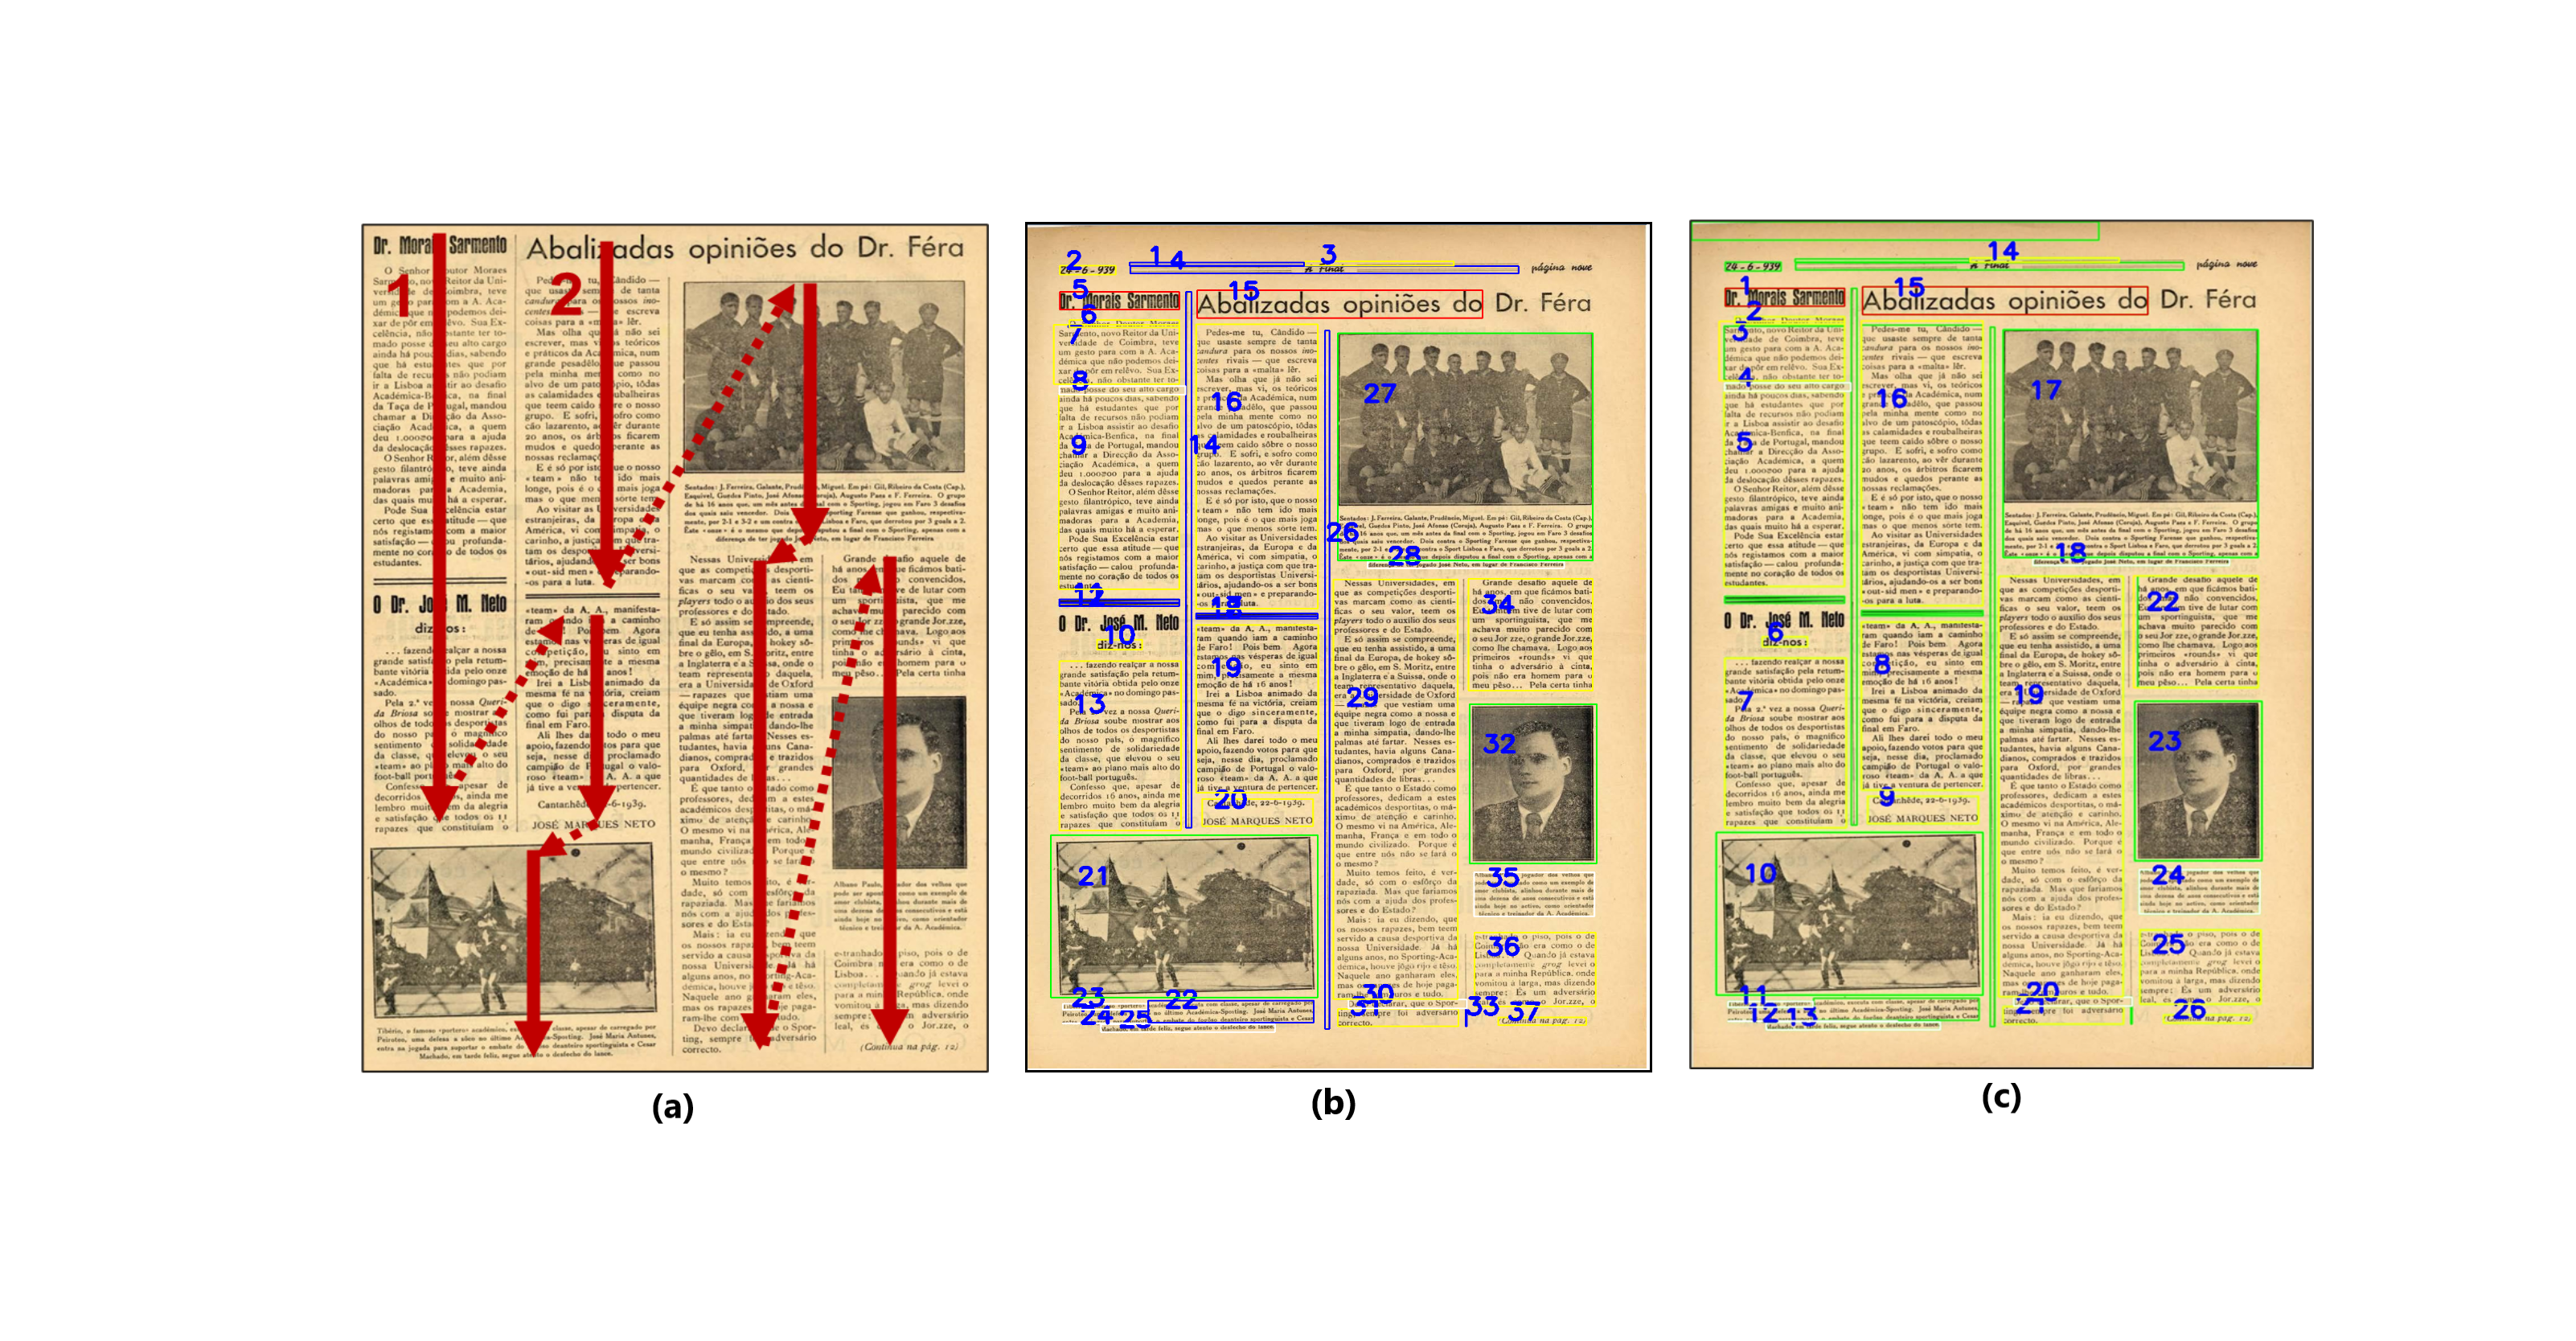
\includegraphics[width=1.5\textwidth]{images/implementacao/algoritmos/comparacao_ordem_leitura.png}
    \caption{Comparação de ordens de leitura: (a) ordem correta; (b) ordem do Tesseract; (c) ordem do algoritmo implementado}
    \label{fig:comp_reading_order}
\end{figure}

Como se observa na imagem \ref{fig:comp_reading_order}, para o exemplo desta página de jornal, a ordem de leitura calculada pelo algoritmo, embora com alguns erros, assemelha-se significativamente mais À correta do que a fornecida pelo Tesseract.



Esta implementação ainda pode ser denotada como \textit{naive} visto ainda incluir pouco contexto na sua lógica. Outras implementações terão de ser experimentadas e comparadas no futuro.

No entanto, este ponto de partida já permite uma extração simples de artigos. Tendo em conta a ordem de leitura e, assumindo que um artigo é sempre inicializado por um título, podemos cortar a sequência ordenada das caixas pelos seus títulos e assim dividir em artigos. A figura \ref{fig:gui_draw_article} é um exemplo disto. É de notar no entanto, que uma posterior ordenação destes artigos poderia ser realizada.

\chapter{Aplicações}
\label{cap_aplicacoes}


Aplicação do resultado principal (exemplos e casos de estudo)

\section{Introdução}

\section{Sumário}
\chapter{Conclusões e trabalho futuro}
\label{cap_conclusao}

Neste capítulo será feito um sumário do trabalho e estudo realizado e uma introspeção sobre o trabalho futuro.

\section{Conclusões}

O projeto atual, propõe a concretização de uma ferramenta para melhorar os resultados de softwares de reconhecimento de caracteres em documentos estruturados antigos, em particular, jornais. Para isto, nesta primeira fase, foram definidos os objetivos principais do trabalho, assim como algumas vias de expansão consoante o desenrolar da sua implementação. Além disso, foi realizado um estudo sobre o estado da arte com base em dois aspetos principais: softwares \acrshort{ocr} e práticas comuns na sua utilização; e exploração sobre trabalhos relacionados a este tema ou técnicas relevantes para a proposta. Com isto, foi possível entender os desafios mais relevantes que se apresentam ao reconhecimento de caracteres, assim como os procedimentos \textit{standard} para os abordar, nomeadamente: pré processamento de imagem, pós processamento de texto, segmentação e métricas de validação; e algumas soluções focadas em tarefas similares ao do atual trabalho. Por último, realizou-se um compilado de algumas tarefas de implementação já realizadas que auxiliaram na perceção dos desafios impostos no tema e ao mesmo tempo uma melhor perceção sobre o funcionamento e capacidade da tecnologia \acrshort{ocr}.

\section{Perspetiva de trabalho futuro}

Partindo do estado atual do projeto, onde uma base de conhecimento do tema já foi concebida, os futuros passos seguirão maioritariamente na componente prática proposta, i.e. a construção das ferramentas para extração de conteúdo de jornais. Como mencionado nos objetivos, abre-se ainda a possibilidade para um aprofundamento na área de criação de léxicos entre versões de uma mesma linguagem para possibilitar a modernização do conteúdo extraído pela ferramenta principal. 
		
\chapter{Planeamento}

\section{Atividades}

\newacronym{rpd}{RPD}{Relatório de Pré-Dissertação}
\newacronym{eda}{EA}{Estado da Arte}

\begin{table}[H]
\begin{center}
\begin{tabular}{| c | c | c | c | c | c | c | c | c | c | c |}
\hline
\textbf{Tarefa} & \textbf{Out} & \textbf{Nov} & \textbf{Dez} & \textbf{Jan} & \textbf{Fev} & \textbf{Mar} & \textbf{Abr} & \textbf{Mai} & \textbf{Jun} & \textbf{Jul}\\
\hline
\textit{Background} e \acrshort{eda} & $\bullet$ & $\bullet$ & $\bullet$ & & & & & & & \\
\hline
Preparação do \acrshort{rpd} & & $\bullet$ & $\bullet$ & $\bullet$ & & & & & & \\
\hline
Contribuição & & & &$\bullet$ &$\bullet$ &$\bullet$ &$\bullet$ &$\bullet$ &$\bullet$ & \\
\hline
Escrita & & & & & & & $\bullet$ & $\bullet$ & $\bullet$ & $\bullet$ \\
\hline
\end{tabular}
\end{center}
\caption{Plano de atividades.}
\end{table}


\renewcommand{\baselinestretch}{1}
\bibliographystyle{plainnat}
\bibliography{dissertation}
\printindex

\appendix
\renewcommand\chaptername{Apêndice}

\part{Apêndices}

\chapter{Trabalho de apoio}
Resultados auxiliares.
\chapter{Detalhes dos resultados}


\begin{figure}[H]
	\centering
	\includegraphics[angle=90,width=0.3\textwidth]{images/resultados/graph_avg_text_conf.png}
	\caption{Valores de confiança média de texto das diferentes pipelines (alargado).}
	\label{fig:graph_avg_text_conf_large}
\end{figure}



\begin{figure}[H]
	\centering
	\includegraphics[angle=90,width=0.4\textwidth]{images/resultados/graph_gt_similiraty_cosine.png}
	\caption{Valores de similaridade do texto (similaridade por cosseno) com GT das diferentes pipelines (alargado).}
	\label{fig:graph_gt_similiraty_cosine_large}
\end{figure}


\begin{figure}[H]
	\centering
	\includegraphics[angle=90,width=0.4\textwidth]{images/resultados/graph_gt_word_hit_ratio.png}
	\caption{Rácios de aparição total de palavras da GT das diferentes pipelines (alargado).}
	\label{fig:graph_gt_word_hit_ratio_large}
\end{figure}


\begin{figure}[H]
	\centering
	\includegraphics[angle=90,width=0.4\textwidth]{images/resultados/graph_gt_unique_word_hit_ratio.png}
	\caption{Rácios de aparição de palavras distintas da GT das diferentes pipelines (alargado).}
	\label{fig:graph_gt_unique_word_hit_ratio_large}
\end{figure}


\begin{figure}[H]
	\centering
	\includegraphics[angle=90,width=0.4\textwidth]{images/resultados/graph_pgt_hit_ratio.png}
	\caption{Rácios de aparição de linhas da Partial GT das diferentes pipelines (alargado).}
	\label{fig:graph_pgt_hit_ratio_large}
\end{figure}


\begin{figure}[H]
	\centering
	\includegraphics[angle=90,width=0.4\textwidth]{images/resultados/graph_pgt_correct_order_ratio.png}
	\caption{Rácios de acerto da ordem das linhas da Partial GT das diferentes pipelines (alargado).}
	\label{fig:graph_pgt_correct_order_ratio_large}
\end{figure}



\begin{figure}[H]
	\centering
	\includegraphics[angle=90,width=0.4\textwidth]{images/resultados/graph_text_block_ratio.png}
	\caption{Rácios de número de blocos de texto relativo à pipeline simples (alargado).}
	\label{fig:graph_text_block_ratio_large}
\end{figure}

\chapter{Listings}
Se for o caso.
\chapter{Ferramentas}
(Se for o caso)

Utilizadores de \Latex\ devem consultar \TUG,
o grupo de utilizadores \tug{\TeX}.

\pagestyle{empty}
\cleartoevenpage
\null
\thispagestyle{empty}
\pagecolor{PANTONECoolGray7C}
\afterpage{\nopagecolor}
\newpage

\begin{backcover}
\thispagestyle{empty}{~\vfill
\noindent
Coloque aqui informação sobre financiamento, projeto FCT, etc. em que o trabalho se enquadra. Deixe em branco caso contrário.
\vfill ~}
\end{backcover}



\end{document}
